% ch-introduction.tex -- what Yuzen is and what it is for
\chapter{はじめに}
\label{ch:introduction}

Yuzen は、基板上の薄い液膜の時間発展を計算するソルバーである。表面張力によるレベリング、重力や
回転による流れ、溶媒の蒸発に伴う膜の濃縮と固化、膜の縁にある接触線の前進・後退を扱う。

C++17 で書かれた研究用のソルバーであり、手作業でインストールする依存関係はない。ケースを一つの
テキストファイルに記述し、一つの実行ファイルを実行すると、ParaView で開ける結果ディレクトリが
得られる。

\section{Yuzen の扱う問題}
\label{sec:intro:what}

Yuzen は、膜厚$h(x,y,t)$に対する長波長近似（潤滑近似）の方程式を、溶質濃度$c$の輸送方程式と
連成させて解く。無次元形で書くと
%
\begin{align}
  \frac{\partial H}{\partial T} &= -\nabla\cdot\Qvec - \Ev\,\hat{E}(H,C) + \hat{S},
  \label{eq:intro-height}\\
  \frac{\partial (HC)}{\partial T} &= -\nabla\cdot\bigl(C\,\Qvec\bigr)
    + \Df\,\nabla\cdot\bigl(\hat{D}(C)\,H\,\nabla C\bigr) + C_S\,\hat{S},
  \label{eq:intro-conc}
\end{align}
%
となる。流束$\Qvec$には、毛管レベリング、分離圧、鉛直方向と面内の重力、遠心力、マランゴニ応力が
含まれる。第一式は液体の移動を表す。第二式は、溶質$HC$を同じ流束で運び、拡散させる。蒸発は溶媒だけを
奪うので、第二式には現れない。蒸発は膜を薄くすることで溶質を濃縮する。ノズルから供給される液体
$\hat{S}$は、到着時の濃度$C_S$で溶質を持ち込む。$C_S$は既定ではその場所の$C$とし、独自の濃度を
与えることもできる。方程式の完全な形は\cref{ch:governing}で導出し、各項は\cref{ch:terms}で説明する。
$C$を膜厚方向に解像するモデルは\cref{ch:concentration}で扱う。

\cref{eq:intro-height}は、膜厚が面内の変化の長さに比べて小さいという近似に基づく。この仮定により、
ナビエ・ストークス方程式は$h$に対する一つの発展方程式に帰着する。そのため、ウェハーの数ミリメートル
だけでなく、塗布したウェハー全体を計算できる。一方で、モデルの限界もこの仮定で決まる。この限界は
\cref{sec:governing:breakdown}にまとめて示す。

\section{考慮できる物理素過程}
\label{sec:intro:physics}

以下の各過程は方程式の独立した項であり、入力ファイルの対応するブロックで有効にする
（\cref{ch:ref-physics}）。ブロックを書かなければ、その項は無効となる。

\begin{itemize}
  \item 毛管圧（ラプラス圧）：表面張力によるレベリング（\cref{sec:terms:laplace}）。
  \item 分離圧：前駆膜上での濡れ、脱濡れ、接触線の移動。平衡接触角に合わせて係数を定める
    （\cref{sec:terms:disjoining}、\cref{ch:wetting}）。
  \item 鉛直方向の重力。平坦でない基板上の流れを含む（\cref{sec:terms:vgravity}）。
  \item 面内重力：傾斜した基板上の流下（\cref{sec:terms:hgravity}）。
  \item 遠心力：スピンコーティング（\cref{sec:terms:centrifugal}）。
  \item 溶質マランゴニ応力（\cref{sec:terms:marangoni}）。
  \item 基板でのナビエすべり（\cref{sec:terms:slip}）。
  \item 溶媒の蒸発。空間分布と前駆膜上での補正を含む（\cref{sec:terms:evaporation}）。
  \item 固定または移動するノズルからの液体の供給（\cref{sec:terms:source}）。
  \item 溶質の輸送。膜厚方向に一様とするモデルと膜厚方向の分布を解くモデルがあり、
    粘度、表面張力、拡散係数の濃度依存性を考慮できる（\cref{ch:concentration}）。
\end{itemize}

\section{適用範囲}
\label{sec:intro:uses}

典型的な応用は、スピンコートしたフォトレジスト、機能性コーティング、乾燥する膜、濡れと脱濡れの問題
である。具体的には、次の場合に Yuzen は妥当な選択である。

\begin{itemize}
  \item 膜が、関心のある面内の構造に比べて薄く、$\As = (L_0/h_0)^2$が大きい。
  \item 流れが粘性的で、慣性を無視できる。
  \item ある瞬間の三次元の速度場ではなく、物理時間で数秒から数分にわたる膜形状の変化を知りたい。
  \item 対象とする物理が、レベリング、乾燥、マランゴニによる筋、回転、接触線の運動の組合せである。
\end{itemize}

一方、慣性が重要な場合、接触線の近くだけでなく至るところで界面の勾配が大きい場合、膜が分裂して
液滴に分かれる場合、膜内部の三次元の流れが必要な場合には適さない。最初の二つは
\cref{sec:governing:breakdown}で定量的に評価している。接触角の較正に用いる小角度近似の誤差は、
\ang{10}で\SI{0.3}{\percent}、\ang{90}で\SI{23}{\percent}である。

\section{計算結果の例}
\label{sec:intro:gallery}

この節の図はすべて、\file{cases/}に同梱したケースを実行し、ソルバーが実際に書き出した出力から
\file{docs/figures/\bk make\_examples.py}で描いたものである。理想化や手作業での描き直しは一切して
いない。ケースを実行すれば、同じ図が得られる。

\begin{figure}[tbp]
  \centering
  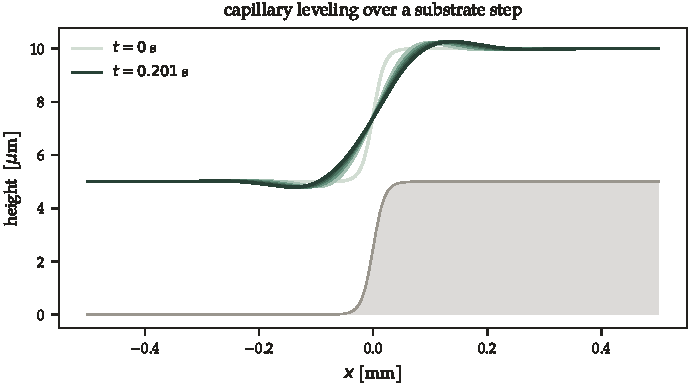
\includegraphics[width=\textwidth]{../figures/leveling-1d.pdf}
  \caption{基板の段差上の毛管レベリング（\file{leveling\_1d\_reg.toml}）。灰色の部分は基板$s$である。
    曲線は\SI{0}{\second}から\SI{0.2}{\second}までの六つの時刻における自由表面$h+s$で、時刻が進むほど
    濃い色で示す。膜は段差に沿った一様な厚さの層から始まり、そのまま平らになるわけではない。曲率によって
    液体が凸の肩から凹の裾へ押し出されるため、段差の下側にくぼみができ、上側に縁が盛り上がる。立ち上がり
    手前の谷と、その先の行き過ぎの組は、四階のレベリング演算子に特有の形である。\cref{ch:governing}では
    この演算子を導出する。\label{fig:gallery:leveling1d}}
\end{figure}

\begin{figure}[tbp]
  \centering
  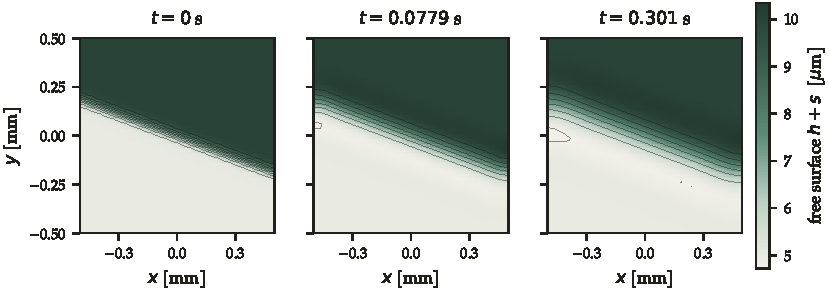
\includegraphics[width=\textwidth]{../figures/leveling-2d.pdf}
  \caption{同じ現象の平面図（\file{allphys\_2d\_reg.toml}）。面内の重力と遠心力の項を含め、すべての項を
    有効にしている。色は自由表面$h+s$を表し、等高線も同じ場から描いている。初期の段差は領域を斜めに横切る
    直線状の縁であり、解はどちらの格子方向にも揃っていない。段差は広い斜面へと広がり、
    \cref{fig:gallery:leveling1d}の谷は閉じた等高線として現れる。\label{fig:gallery:leveling2d}}
\end{figure}

\section{モデル}
\label{sec:intro:models}

次元と濃度モデルの組合せとして、四つのモデルを実装している。モデルは\key{Physics.ConcField.Model}と
\key{Grid.Dimension}の二つのキーで選ぶ。

\begin{yzntable}{四つのモデル\label{tab:models}}{@{}L{0.13\textwidth} L{0.13\textwidth} L{0.64\textwidth}@{}}
\textsf{\bfseries モデル} & \textsf{\bfseries 次元} & \textsf{\bfseries 説明}\\ \midrule
\val{"WM"} & \val{"xh"}  & 1 次元の稜線。濃度は膜厚方向に一様 \\
\val{"WM"} & \val{"xyh"} & 2 次元の平面図。濃度は膜厚方向に一様 \\
\val{"CZ"} & \val{"xh"}  & 1 次元の膜。濃度を膜厚方向に解像、$c(x,z,t)$ \\
\val{"CZ"} & \val{"xyh"} & 2 次元の膜。濃度を膜厚方向に解像、$c(x,y,z,t)$（擬似 3 次元） \\
\end{yzntable}

「鉛直一様（well mixed）」とは、溶質濃度を膜厚方向に一様とみなすことをいう。\val{"CZ"}モデルは濃度を
膜厚方向に解像する。その代わり$z$方向の格子が必要になり、物理項が二つ使えなくなる。分離圧と湧き出し項を
使えないため、接触線の問題には\val{"WM"}を用いる。両モデルの比較と、鉛直一様の仮定が成り立たなくなる
条件は\cref{ch:concentration}で述べる。

\section{計算の流れ}
\label{sec:intro:pieces}

Yuzen の計算は、一つの入力ファイルを読む一つのプロセスで行う。\textbf{一台の計算機上の一つの
プロセス}である。Yuzen は OpenMP で並列化しており、MPI には対応していない。そのため、解ける問題の
大きさは一つのノードのメモリーで制限される（\cref{ch:parallel}）。

\begin{enumerate}
  \item 入力ファイル（TOML 文書）を解析し、整合性を検査する。入力が整合しない場合は、計算を始める前に
        中断する。
  \item 次元をもつ入力を内部の無次元形に変換する。実際に用いたスケールは、標準出力の実行ログに
        表示する。
  \item \key{JobName}にちなんだ名前の結果ディレクトリを作り、入力ファイルをそこにコピーする。
        そのため、結果ディレクトリだけで計算条件を特定できる。
  \item ソルバーはニュートン・カントロビッチ反復で膜厚を進め、同じ反復の中で濃度の方程式も解く。
        これを、終了時刻に達するか、膜が乾ききるか、解が定常になるまで続ける。
  \item 場、履歴、時間刻みごとの診断量を、それぞれ独立した間隔で書き出す。
\end{enumerate}

膜厚の方程式は、時間方向にクランク・ニコルソン法で進め、項ごとに組み立てた解析的なヤコビアンを用いる。
濃度の方程式はニュートン反復の内側で半陰的に解く。そのため、収束した状態は両方の方程式を同時に
満たす（\cref{sec:time:coupling}）。時間刻みは局所打ち切り誤差の推定に基づいて適応的に決める。線形
ソルバーのバックエンドとして Eigen と AMGCL の二つを、共通のインターフェースのもとで用意している
（\cref{ch:linearsolver}）。

\section{再現性}
\label{sec:intro:repro}

コードの設計を左右する性質が二つあるので、最初に述べておく。

第一に、Yuzen の結果は OpenMP のスレッド数によらず\emph{ビット単位で一致する}。例外は\val{"amgcl"}
バックエンドで、このことは文書に明記している。テストスイートはこの一致を検査し、\code{ctest}はスイート
全体を一スレッドと四スレッドで再実行する。この性質を支える四つの実装上の工夫と、そのどれも「整理」
してはならない理由は\cref{ch:reproducibility}で説明する。

第二に、\cref{ch:verification}の数値はすべてリポジトリから再現でき、再現するためのコマンドを数値の
隣に示している。確認していない事項は\cref{ch:notverified}に挙げる。

\section{ライセンスと引用}
\label{sec:intro:license}

本マニュアルは Yuzen 1.0 について記述する。バージョン番号が入力ファイルと結果について何を保証するかは
\cref{ch:policy}に、このリリースの内容は\cref{ch:revisions}に示す。

Yuzen は Apache License, Version 2.0 のもとで配布している。\file{LICENSE}と\file{NOTICE}を
参照されたい。同梱したサードパーティーのコードは doctest（MIT）と toml++（MIT、手元での修正を一つ
含む）である。Eigen（MPL-2.0、必須）と AMGCL（MIT、任意）はビルド時に取得する。各バージョンと
toml++ への変更内容は\file{THIRD\_PARTY\_NOTICES.md}に記載している。研究成果の公表に Yuzen を
用いた場合は、\file{CITATION.cff}に示す形式で引用されたい。

コードとそのコメント、本マニュアルの第III部から第V部のもとになった\file{docs/}の原典文書、本マニュアルの
原典（英語版）は、いずれも英語で書かれている。
